\newpage
\section{\framework{} Methodology}
\label{sec:methodology}

We now provide the methodology to achieve the goal of deceiving user data fed to the apps without rooting the device or altering the source of the apps.

\subsection{Background on Hooking}
In Android, a typical user does not have permission to modify the apps or OS behaviour. However, \textit{hooking} into OS and apps is one of the most practical options to alter the behaviour of an app. Hooking is a technique of code modification that changes the behaviour of the original code running sequence by inserting instructions into the code segment. 

Hooking can be performed in two ways: statically and dynamically. The static hooking technique injects hooks before app execution by altering the byte code of the app or by injecting custom shared libraries. However, static hooking causes permanent alteration and can be detected by an app using a digital signature. 

Dynamic hooking technique applies ``hooks'' at runtime by modifying the code stored in volatile memory (temporary modification), allowing hooking decisions based on the runtime environment. Android's Dalvik VM utilizes Dynamic Linkers' ``virtual method table'' to jump to the memory location on a method call, hence \textit{Call Diversion} can be employed to inject hooks in the hooked method lookup table entry. 

\begin{figure}[t]
    \centering
    \begin{subfigure}{0.48\linewidth}
        \vspace{7mm}
        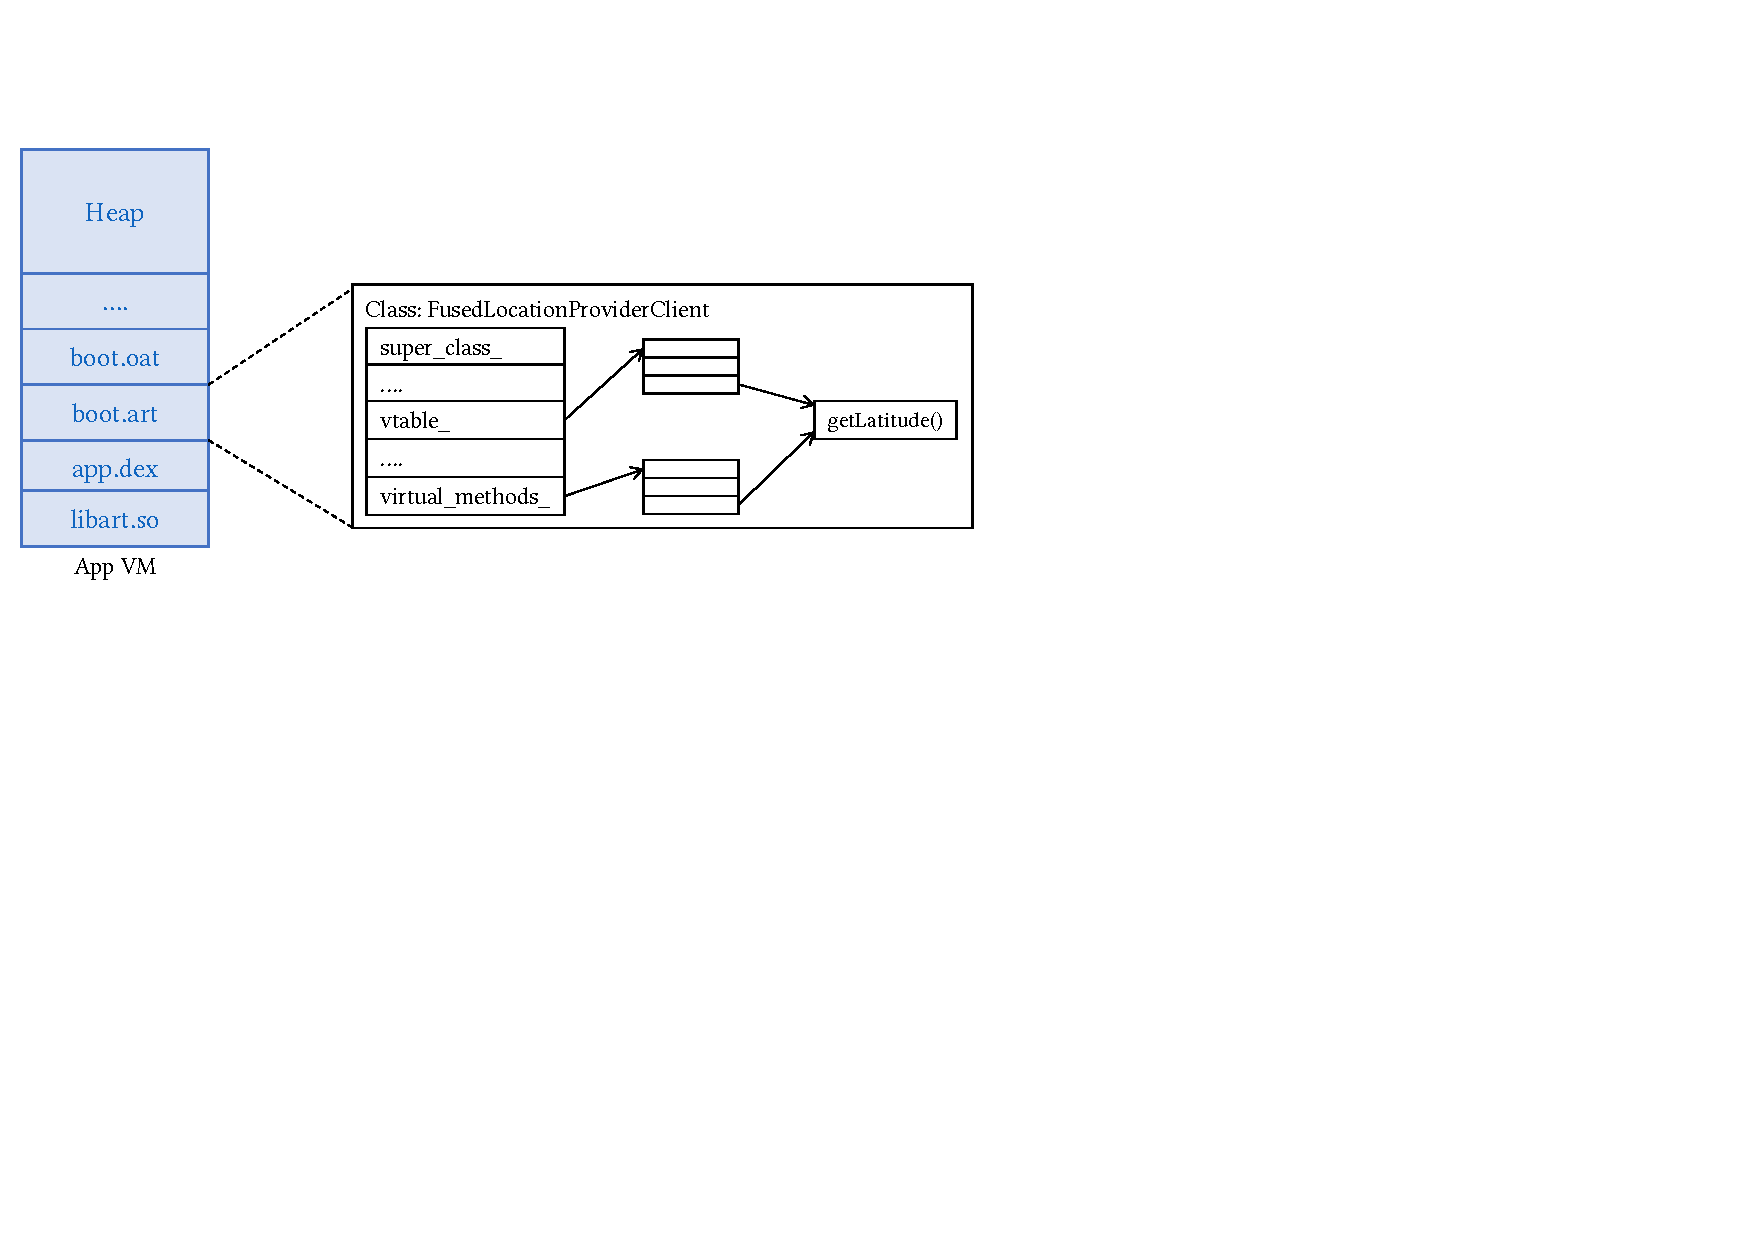
\includegraphics[width=\linewidth]{Figures/Background/virtual_memory_without_deceiver.pdf}
        \caption{Original method call.}
        \label{fig:vrtulMemMthdCall_woFr}
    \end{subfigure}
    \begin{subfigure}{0.48\linewidth}
        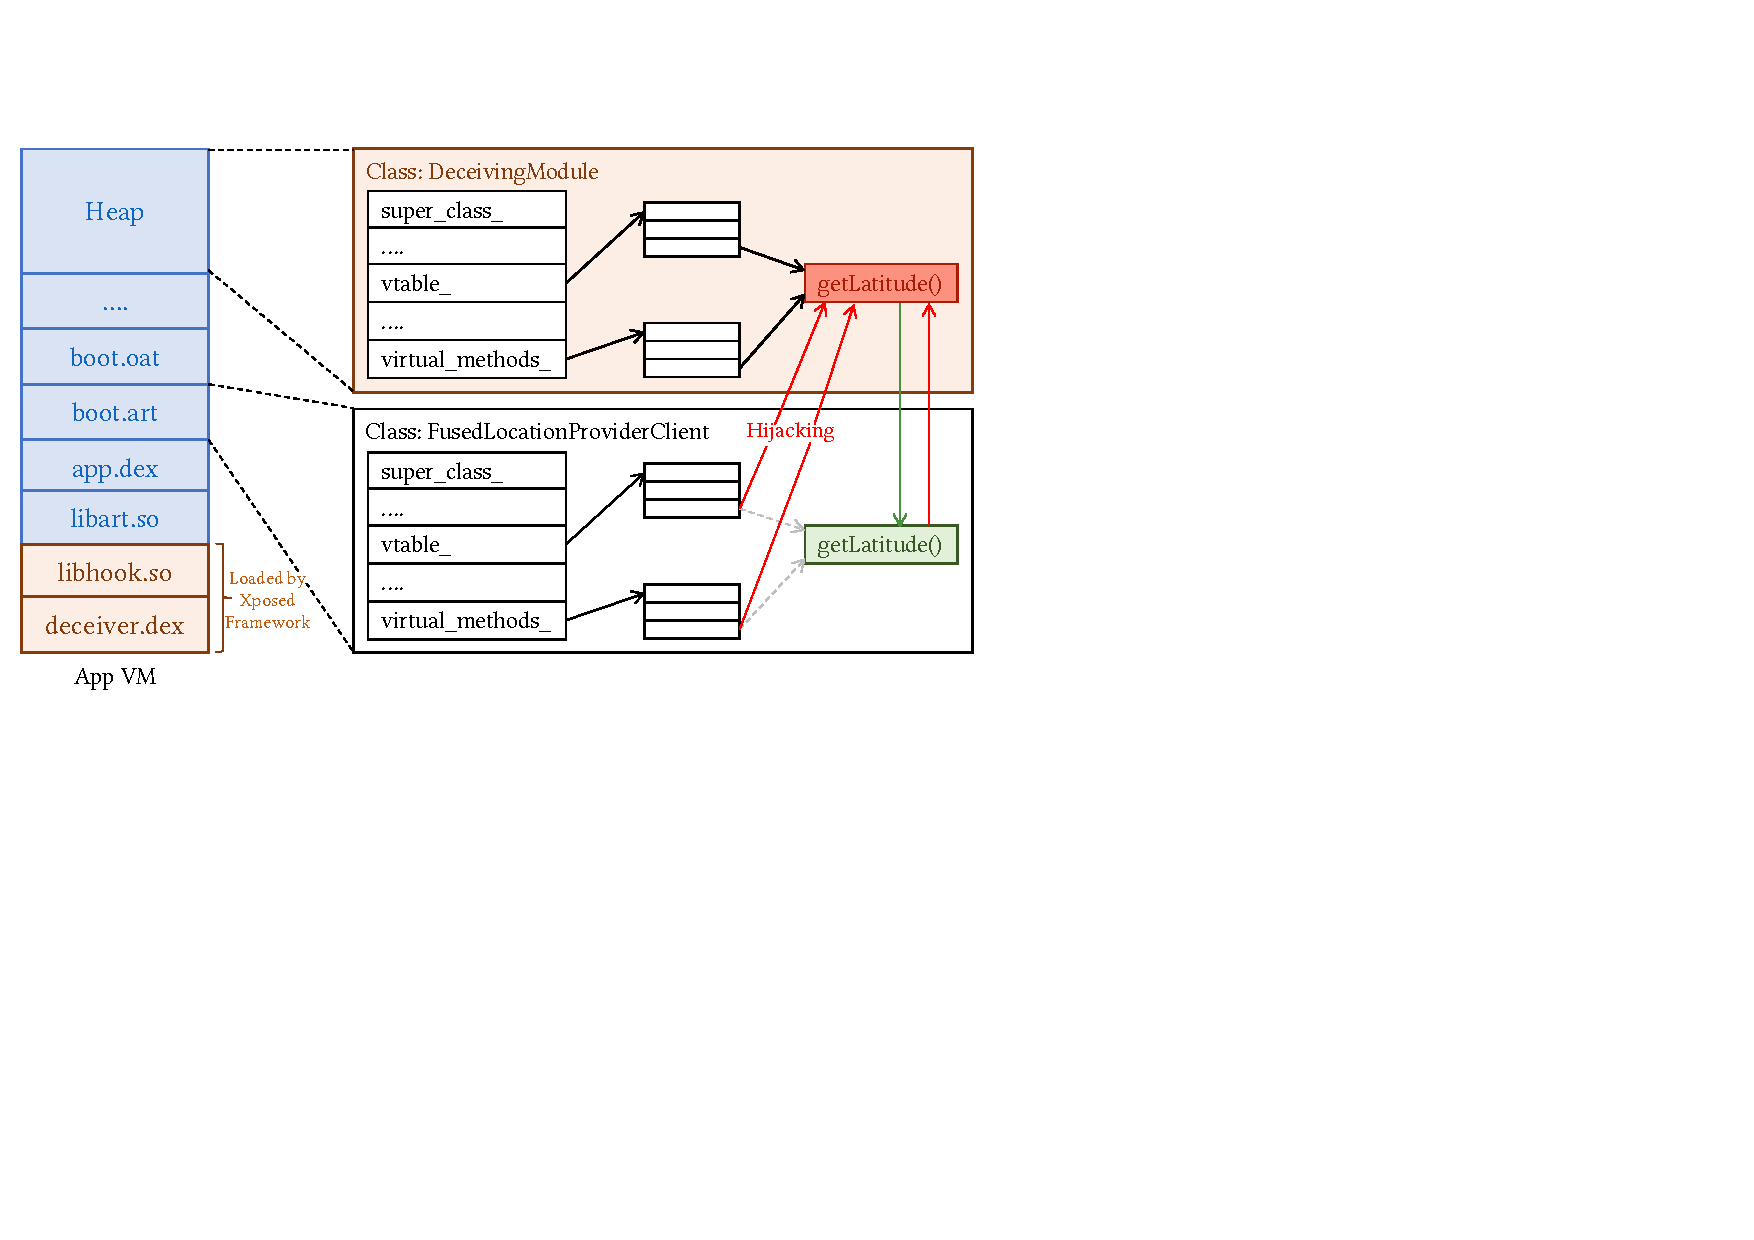
\includegraphics[width=\linewidth]{Figures/Background/virtual_memory_with_deceiver.pdf}
        \caption{Method call with \framework{}.}
        \label{fig:vrtulMemMthdCall_wFr}
    \end{subfigure}
    \caption{Example illustrating how the Xposed module class method hijacks the original method call.}
    \label{fig:vrtulMemMthdCall}
\end{figure}

In Figure \ref{fig:vrtulMemMthdCall}, we present an overview of dynamic hooking in Android using the \texttt{Location.getLatitude()} method. Figure \ref{fig:vrtulMemMthdCall_woFr} illustrates the conventional process of method call jumps. The virtual memory of the target app encompasses the heap space and various files loaded by the \textit{Zygote} process to initiate the app process. Zygote is a process started by the Android Framework during the OS boot. It is a template process preloaded with Java-shared libraries in memory, responsible for launching apps and services. 

The \texttt{boot.oat} and \texttt{boot.art} files serve as boot images to speed up the boot proces containing frequently used class source code and the pre-initialized heap respectively. The heap of the target class is stored in the \texttt{boot.art} file. The Dalvik Executable code of the app and the shared libraries are stored in the \texttt{app.dex} and \texttt{libart.so} respectively. When the target method is invoked by the app, the existence of the target class is checked in the \texttt{boot.art} file. If the class is found, the addresses of the target methods are determined using the virtual tables stored in the heap. Consequently, the execution jumps to the identified address.

% In contrast, 
Figure \ref{fig:vrtulMemMthdCall_wFr} depicts the process of hooking. The hooked application's virtual memory is loaded with the \texttt{libhook.so} shared library by the hooking module, facilitating the hooking operations. Subsequently, the hooks defined by the hooking app (\texttt{hook.dex}) are loaded by the hooking module as Dalvik Executables (same as app code). Upon completion, \texttt{libhook.so} intervenes and loads the hooking classes into the app's heap space, modifying the entries of the target class virtual tables with the addresses of the hooking class methods. Consequently, when the app calls the hooked methods, the calls are redirected to the hooking class methods instead of the original methods. Finally, the original method is invoked by storing its address at the end of the hooking method.

% \begin{lstlisting}[caption={Kotlin code to deceive Clipboard permission data with the data defined by user in \textit{Deceit} policies.},label={lst:clipboardDeceiver},language=Kotlin,float=*]
class SpoofingModule: IXposedHookLoadPackage {
    companion object {
        fun getClass(clsName: String): Class<*> = Class.forName(clsName, false, lpparam.classLoader)    
    }
    
    @Throws(Throwable::class)
    override fun handleLoadPackage(lpparam: XC_LoadPackage.LoadPackageParam) {
        hookAllMethods(getClass(ClipData.CREATOR.javaClass.name), "createFromParcel", XC_MethodHook() {
            @Throws(Throwable::class)
            override fun beforeHookedMethod(param: MethodHookParam) {
                val uri = Uri.parse("content://com.xposedModule.provider/deceitSettings")
                val cursor = context.contentResolver.query(uri, null, null, null, null) ?: return
                val blockClipboard = cursor.getInt(cursor.getColumnIndex("blockClipboard")
                cursor.close()
                if(blockClipboard) param.result = null
            }

            @Throws(Throwable::class)
            override fun afterHookedMethod(param: MethodHookParam) {
                param.result ?: return
                val uri = Uri.parse("content://com.xposedModule.provider/deceits")
                val cursor = context.contentResolver.query(uri, null, null, null, null) ?: return
                val clipboardLabel = cursor.getString(getColumnIndex("clipboardLabel")) ?: "dummyLabel"
                val clipboardText = cursor.getString(getColumnIndex("clipboardText")) ?: "dummyText"  
                cursor.close()
                param.result = ClipData.newPlainText(clipboardLabel, clipboardText)
            }       
        })   
    }
}
\end{lstlisting}

\subsection{Hooking on Non-Rooted Device}

We found that the most suitable solution to deceive user data is app hooking. However, on non-rooted devices, users are restricted from accessing the root and hooking various processes within the system. To gain hooking capabilities, root access to the \textit{Zygote} process is required. 

For this, we utilize \textit{adb} (\textit{Android Debug Bridge}), a command-line tool typically utilised for debugging apps, but also capable of controlling Android devices and executing shell commands. \textit{adb} provides user-installed apps with privileged access to the system APIs. This access is limited till the device is in an active connection with the \textit{adb} tool. This limitation is futher tackled by the Shizuku service by exploiting \textit{adb} shell access. Shizuku provides privileged access to system APIs to user-installed apps by running a dedicated process with shell-level permissions, acting as a proxy between the apps and the OS. This level of access is sufficient for hooking the target apps to spoof the user data. 
%The users need to restart the Shizuku service after every device reboot. 

Employing the Shizuku service, we use LSPatch, an Xposed framework for non-rooted devices, for hooking the target apps by injecting the hooks into app processes. This allows users to define the required app behaviour within the Xposed module to make the target app execute their desired actions. Both the Shizuku service and LSPatch are open-source and user-controlled, they only grant root privileges to the modules and apps chosen by the user, ensuring that the attack surface remains unchanged.

\subsection{Spoofing User Data with Hooking}

In Listing \ref{lst:clipboardDeceiver}, we present the approach employed to spoof the Clipboard data with custom spoofed data by hooking. Typically, the app retrieves clipboard data by calling the \texttt{ClipboardManager.getPrimaryClip()} method. However, to modify the result of this method, multiple other methods need to be hooked. Alternatively, a more efficient approach involves hooking \texttt{ClipData.CREATOR.createFromParcel()} method, as ultimately, this method is called by the former method to return the clipboard data. To hook this method, we utilise Xposed's \texttt{handleLoadPackage()} in Line~7.

Using this mechanism, the Clipboard data can either be blocked or modified before feeding into the target apps. In the before hook, Line 11-15 lists the code for blocking the clipboard data from feeding into the target apps. Using \textit{ContentProvider} the Xposed module is gathering the user's choice on blocking the clipboard data in Line 11-13. And then in Line 15, if the user opts for blocking the clipboard data, then the resultant part of the function call is updated with null object. This blocks the original method call and execution returns back to the method from where the call for the hooked method is made. 

Similarly, in the after hook, i.e. Lines 20-26, the clipboard data is deceived as plain text data as per the user policy. The user-defined deceived data is fetched from the \textit{ContentProvider} in Line 21-24. And then in Line 26, the result of the method call is updated with a new \texttt{ClipData} object initialised with fetched deceived result.

\framework{} offers diverse policies for deceiving various permissions. For instance, one policy for spoofing camera permission involves blurring the image when the app is operating in the background. In this scenario, \framework{} utilizes the \texttt{ActivityManager} to determine whether the target app is running in the background or not. If it is found to be running in the background while accessing the camera permission, \framework{} blurs the frames supplied to the app by manipulating the pixels. Another intriguing policy employed by \framework{} involves providing a noise audio fed if an app unnecessarily requests Audio permission.

\subsection{\framework{} and its Robustness}
In this section, we present \framework{}'s mechanism to achieve the functionality of spoofing the user data fed into other apps and discuss its performance against real-world apps highlighting its robust nature.

\mysubsubsection{Robust Mechanism} 
By utilising dynamic hooking, \framework{} effectively manipulates user data in other apps by modifying the source code stored in volatile memory, thus avoiding permanent alterations on disk. As a result, the injected hooks cannot be detected using APK signatures or Google's Play Integrity API, making \framework{} resilient against these security measures. Moreover, \framework{} follows a methodology of spoofing user data instead of outright revoking permissions based on context. This approach ensures that \framework{} remains crash-proof, providing a reliable and robust solution.

\mysubsubsection{Spoofing Real-world Apps}
The capability of \framework{} against real-world apps in protecting user privacy by spoofing was explored using 50 real-world apps downloaded from the Google Play Store, and 20 pre-installed Android apps. All permissions requested by the apps were granted beforehand, and the apps were subjected to 20 minutes of manual usage. All experiments were conducted on a \textit{Samsung Galaxy M21} smartphone with a 2.3 GHz octa-core processor and 4 GB of RAM running Android 12. The outcomes were documented for each permission, taking into account visual confirmation of spoofed user data and the logs captured by \framework{}.

The heatmap depicted in Figure \ref{fig:intro_heatmap} provides an overview of the \framework{}'s performance when applied to the most popular apps on the Google Play Store. The dark green region of the heatmap signifies the successful deception of permissions for corresponding Android apps. The light green, orange, and red regions indicate permissions that were not requested, not utilized, and could not be deceived, respectively. 
% 531, 147, 41, 678, 73.85% -> 78.32%, 20.44 -> 21.68%

Out of the 678 permissions requested by 70 apps, the \framework{} achieved a \textbf{78.32\%} success rate in spoofing user data. We could not ascertain the deception for 21.68\% of the permissions because although they were granted to the app, they were not explicitly requested during the experiments. These encouraging results demonstrate the robustness of the \framework{}'s mechanism and design in real-world scenarios as none of the apps crashed and functioned as expected.

\begin{figure}[t]
    \centering
    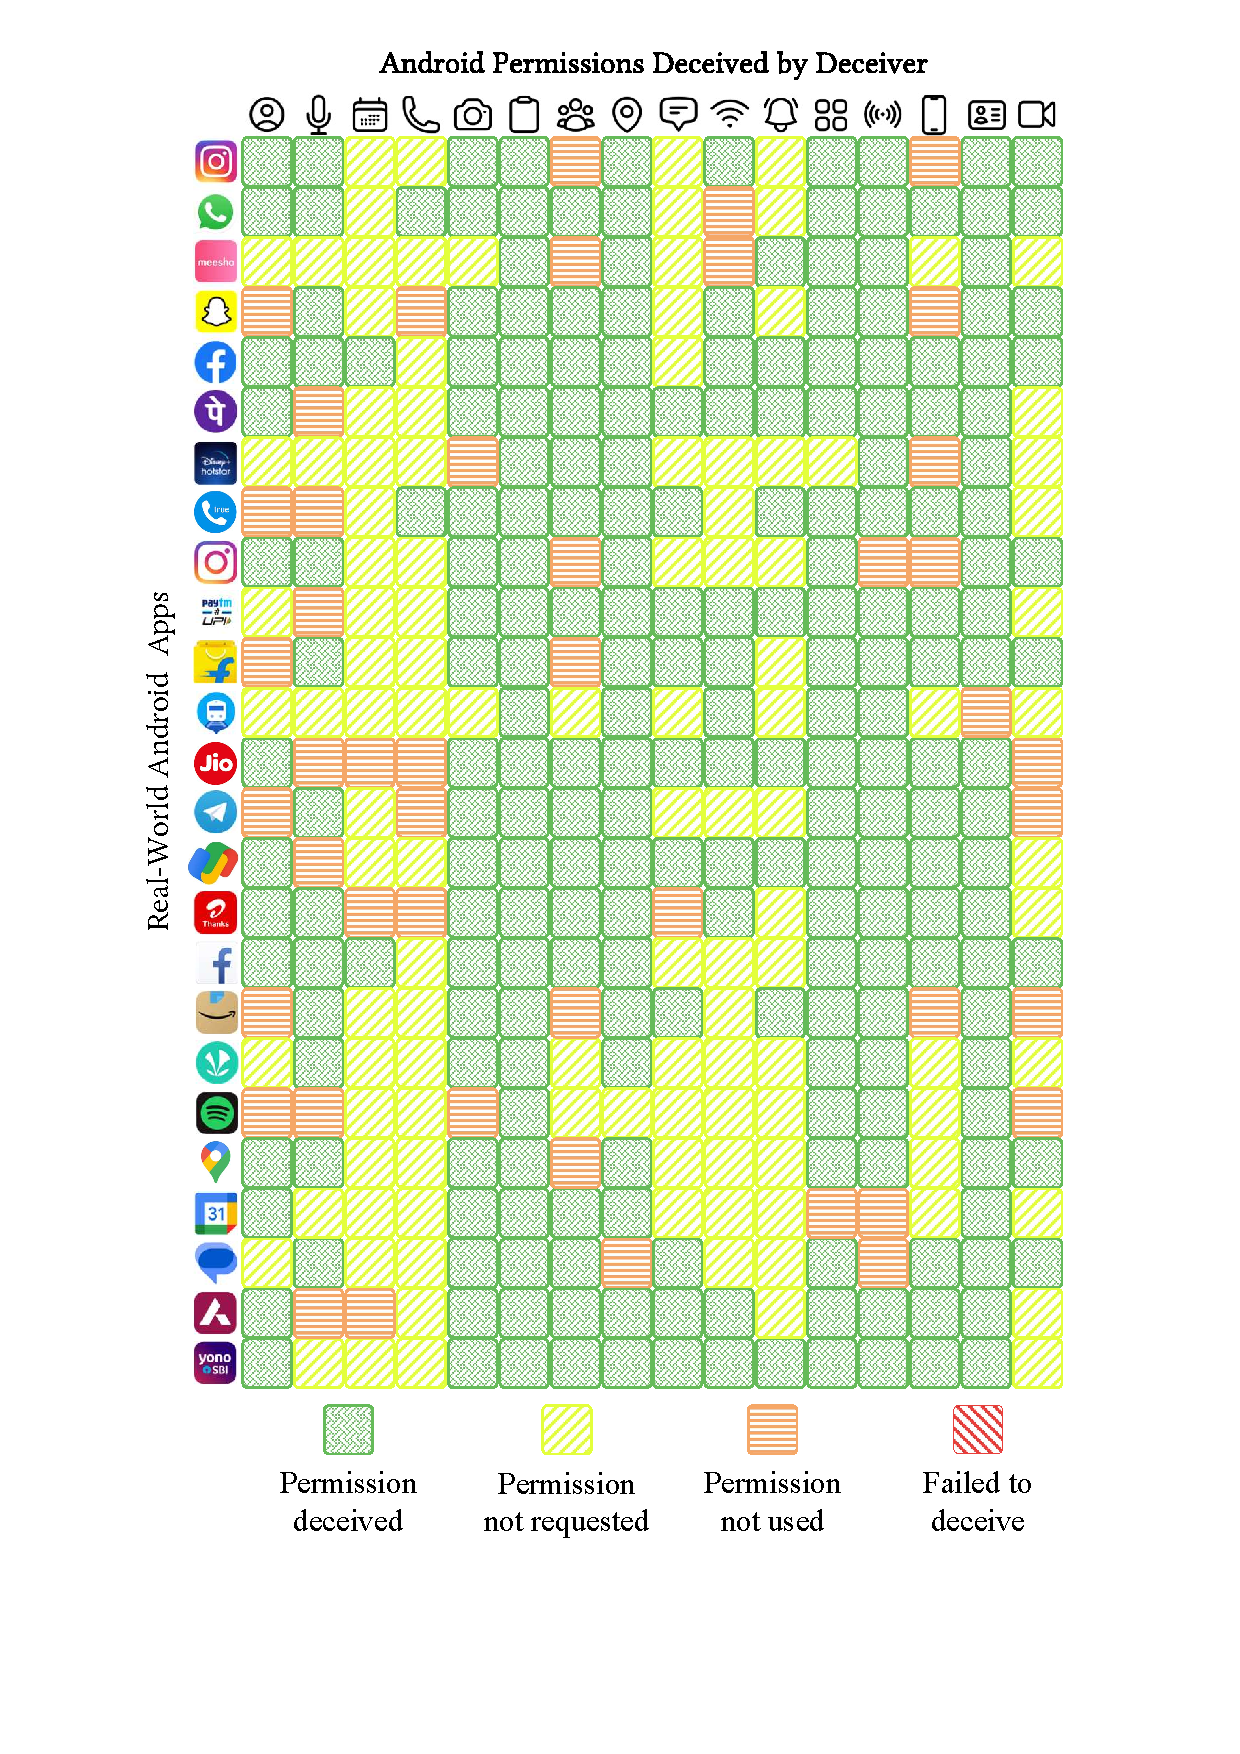
\includegraphics[width=0.6\linewidth]{Figures/Introduction/heatmap.pdf}
    \caption{Heatmap illustrating status of user data deceived for various popular apps by \framework{}.}
    \label{fig:intro_heatmap}
\end{figure}

\mysubsubsection{Hooking Hidden APIs} 
Certain permissions such as sensors, involve method calls returning instances of \textit{Android Non-SDK Interfaces} classes also known as \textit{Hidden APIs} like \texttt{InputSensorInfo}. Accessing these Hidden APIs is restricted for \textit{JNI} and \textit{Java Reflections}. \framework{}'s hooks corresponding to Hidden APIs bypass these restrictions and instantiate classes with deceived data using the \textit{LSPlant}. Out of 78.32\% successfully deceived user data, 23.16\% were deceived by hooking hidden APIs.

\mysubsubsection{Isolation} \framework{} requests the \textit{Query All Packages} permission to facilitate and simplify its privacy protection functionalities which is a non-runtime (normal) permission and the only permission requested by \framework{}. Notably, \framework{} operates offline, severing any external connections and isolating itself from the internet, establishing a secure and trustworthy environment.
